\subsection{Backend}
\label{arquitecura:global_backend}
Plantejat i desenvolupat com una API Rest que dóna accés als recursos necessàris dins de la base de dades, a través de rutes (o \textit{endpoints}) definides als controladors.\\
\newline L'accés a les dades es fa a través d'HTTP, fent ús dels mètodes \textit{Get}, \textit{Post}, \textit{Put} i \textit{Delete}, amb un funcionament similar al \textit{CRUD}\footnote{\textbf{C}reate \textbf{R}ead, \textbf{U}pdate i \textbf{D}elete} d'una base de dades, però a nivell de recurs.\\
\newline Pel que fa a l'arquitectura pròpiament dita, no se n'aplica una de concreta.\\
Per contra, fa ús de tot un seguit de conceptes d'enginyeria del \textit{software} com \textit{clean architecture} i \textit{SOLID}  que tenen com a objectiu la producció d'un codi net, mantenible i sobre tot, ben estructurat.\\
\subsubsection{Clean Architecture}
\label{arquitectura:back_clean}
\begin{figure}[h]
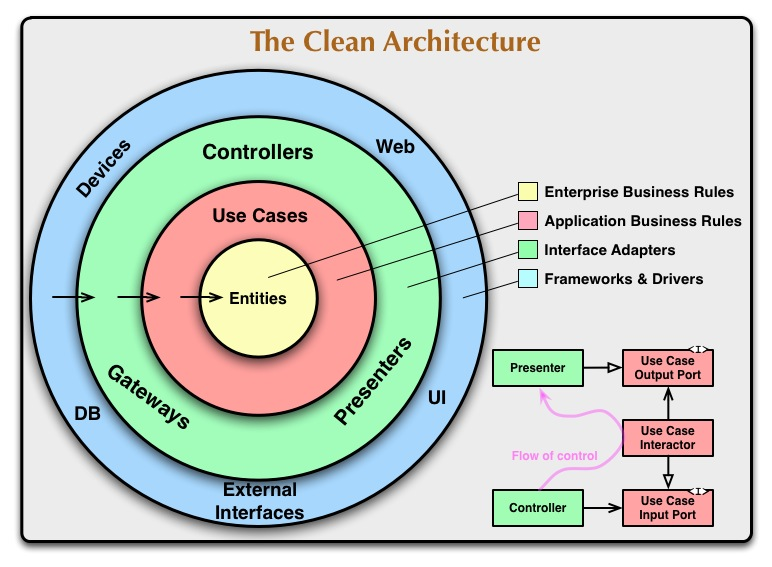
\includegraphics[scale=0.4]{sections/arquitectura/cleanArchitecture.jpg}
\centering
\caption{Clean Architecture}
\label{fig:clean_architecture}
\end{figure}
La figura anterior (Figura \ref{fig:clean_architecture}), ens presenta un model conceptual que rep el nom de \textit{clean architecture}\cite{clean}.% on les diferents capes són independents les unes de les altres, de tal forma que caldrà aplicar tot un seguit d'\textit{adapters} entre capes per poder comunicar-se entre elles.\\
%\newline La capa més interna, no coneix a la capa més externa i viceversa. Aqust fet, provoca una atomicitat tant a nivell conceptual com a nivell de codi bastant notable. \\
%A la llarga, l'atomicitat i el poc solapament aconseguits d'aplicar la filosofía \textit{clean architecture} serà clau per a un bon escalat del projecte.\\
El primer que s'ha de tenir en compte quan es parla d'aquesta arquitectura, és que es regeix pel que s'anomemena \textit{Dependency rule}, segons la qual les capes internes no poden comunicar-se amb les capes externes.\\
\newline Gràcies a aquesta estructura, la lògica de negoci sempre és independent del \textit{framework}, de com s'obtenen o es mostren les dades o altres factors externs.\\
\newline SOLIDi s'ha estructurat el projecte de forma apropiada, no s'ha de patir per si en un futur es canvien tecnologies o llibreries, la lògica de negoci continuarà funcionant exactament igual.
\clearpage
%\newline D'aquesta forma, s'aconsegueix un codi atomitzat, fàcil de mantenir donat el poc solapament que hi ha entre els diferents components del projecte, i amb components fàcilment substituïbles.\\
\subsubsection{S.O.L.I.D}
\label{arquitectura:back_solid}
\cite{solid} És l'acrònim de:
\begin{itemize}
    \item \textit{\textbf{S}ingle responsability}
    \item \textit{\textbf{O}pen close}
    \item \textit{\textbf{L}iskov substitution}
    \item \textit{\textbf{I}nterface segregation}
    \item \textit{\textbf{D}ependency inversion}
\end{itemize}
Els cinc punts anteriors, són un seguit de convencions i idees enfocades a la producció d'un codi net, estructurat i fàcil de mantenir.\\
\newline Per aconseguir-ho, treballa amb idees tal com la responsabilitat única de les classes, classes obertes a l'extensió, però no a la modificació, injecció de dependències, ús de interfícies a mode de contracte, etc.\\
\newline Són tot un seguit de regles que funcionen perfectament amb les idees presentades anteriorment referents a la \textit{Clean Architecture}
\subsubsection{Base de dades}
Tot i que ha patit diversos canvis al llarg del desenvolupament del projecte, el model final de la capa de persistència queda tal que:
\begin{figure}[h]
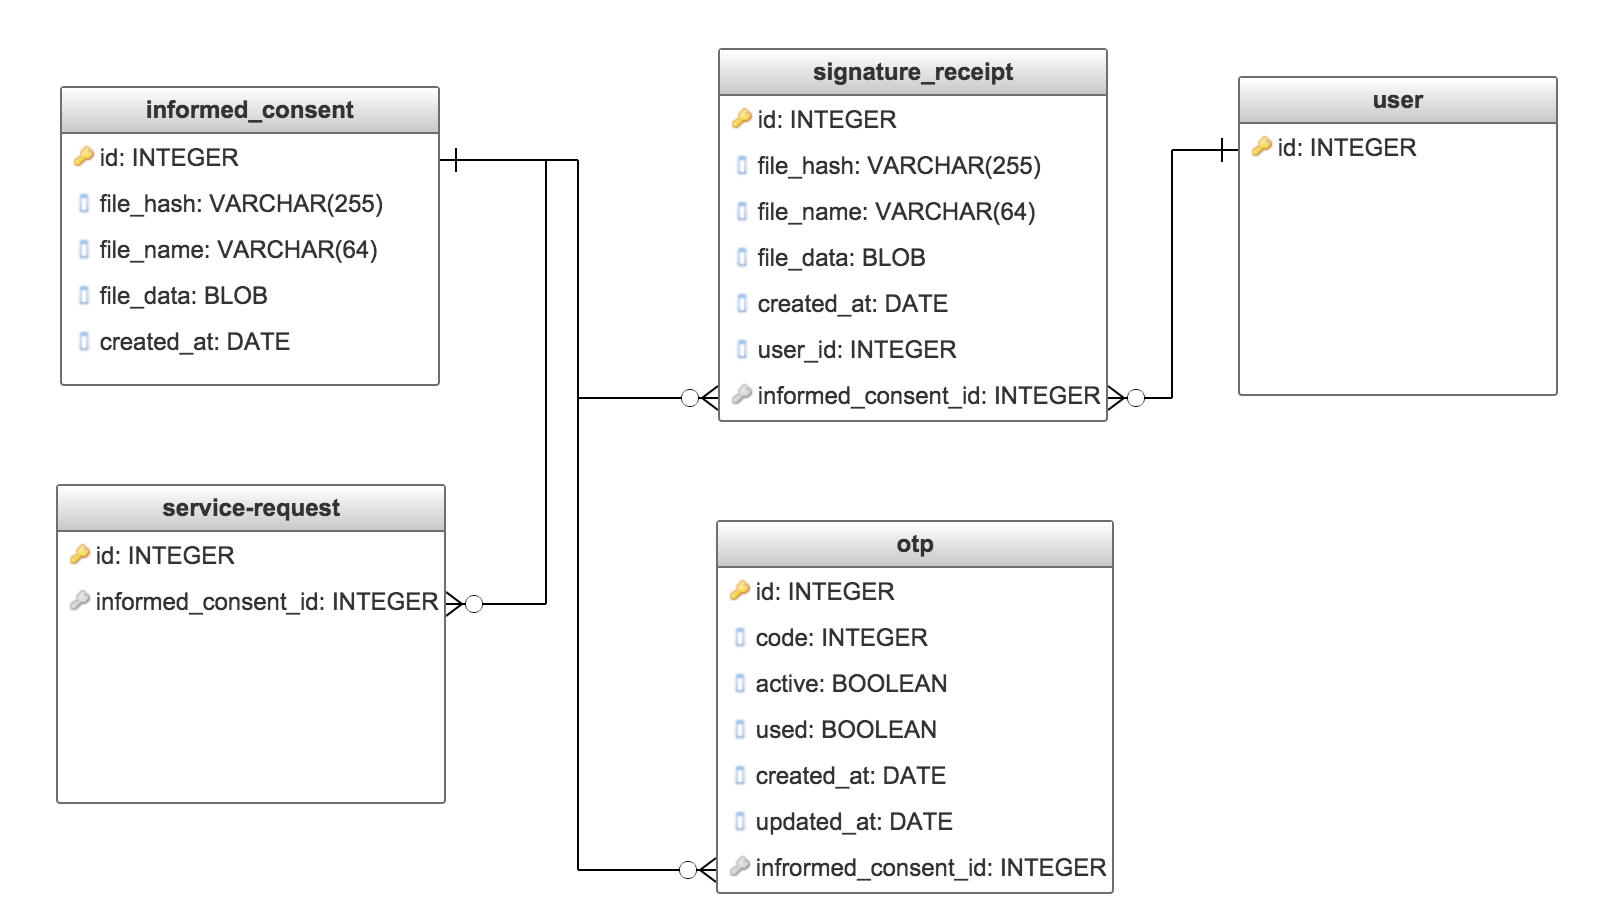
\includegraphics[scale=0.4]{sections/arquitectura/database_model.png}
\centering
\caption{Model de base de dades}
\label{fig:database_model}
\end{figure}
%\begin{itemize}
%    \item Servir les dades al \textit{frontend} sota demanda.
%    \item Realitzar la comunicació amb els serveis externs quan el context això ho demani.
%\end{itemize}

%El \textit{backend} és, en escènica una API Rest que serveix els diferents recursos emmagatzemats a la base de dades (CRUD) per a servir les necessitats que sorgeixin des del \textit{frontend}.\\
%Alhora, realitza la comunicació amb serveis de tercers com \textit{OriginStamp} i \textit{FreeTSA}, necessaris per a garantir el no repudi dels consentiments informats i generats per una segona API privada encarregada de generar tant els consentiments com el comprovant de signatura.\\
%\newline A continuació veurem amb més detall cada un dels components que formen el \textit{backend}:

%\subsection{Nucli}
%Anomenem \textit{nucli} a la API rest a la que el \textit{frontend} llança les diferents crides.
%Aquesta api és un mòdul desenvolupat amb \textit{Symfony}.\\
%\newline \textit{Symfony} és una de les "grans" opcions dins de la extensa llista de \textit{frameworks PHP} existents; alhora que és un dels més emprats per als desenvolupadors per les seves característiques i facilitats, conta amb un renom afegit per ser l'elecció base per a grans projectes com podrien ser el gestor de contingut \textit{Drupal}\footnote{https://www.drupal.org} i \textit{phpBB}\footnote{https://www.phpbb.com/}, un CMS orientat a la creació de fòrums.\\
%\newline Entre les característiques destacades, podem trobar la facilitat d'estructurar el codi, donada la seva clara orientació cap a una arquitectura MVC, així com la re-usabilitat del mateix, sempre i quan es faci ús de bones pràctiques. A tot aixó, \textit{Symfony} conta amb una característica afegida, que també podria ser considerada una facilitat, que és l'ús d'un gestor de dependències per a \textit{PHP} anomenat \textit{Composer}.\\
%De la mateixa manera que hem vist anteriorment al el \textit{frontend}, concretament amb \textit{node.js} i \textit{npm}, \textit{Comsposer} llegeix del fitxer \textit{composer.json} per tal d'instal·lar les dependències del projecte sense necessitat de fer-ho d'una en una, i d'aquesta forma facilitar-ne la migració i el treball col·laboratiu.\\
%\newline Com a característiques de \textit{Symfony}, cal destacar \textit{Doctrine}, un ORM que permet al desenvolupador abstreure's de la gestió de base de dades i la sintaxi del llenguatge SQL i tractar-ne les taules com a classes \textit{PHP} anomenades Entitats, amb tot el que això ofereix.\\
%\newline A nivell de codi, \textit{Symfony} ofereix tot un seguit d'eines pròpies que faciliten i alleugeren el desenvolupament de l'aplicació. Alhora, compta amb una comunitat molt forta i abundant que aporta coneixement i eines alternatives a les incloses al mateix \textit{framework}, que aporten alternatives d'allò més interessants i potents que faciliten i enriqueixen encara més el desenvolupament.\\
%\newline Tornant al context del TFG pròpiament dit, aquest component serveix com a intermediari entre el \textit{frontend} i la capa més purament de dades de tot el global de l'aplicació, la base de dades. \\
%\newline Una API rest que serveix que permet al \textit{frontend} demanar dades i enmagatzemar-ne

%\subsection{Generació de documents}
%Aquest component ha patit diversos canvis al llarg del desenvolupament del projecte, no obstant en posteriors capítols d'aquest Treball de Final de Grau es donaran detalls dels canvis que hi han soegit durant el desenvolupament; de moment es comentarà el disseny final d'aquest integrant del \textit{backend}.\\
%\newline Per a la creació dinàmica de documents, s'ha optat per crear una segona API Rest independent a la descrita a l'apartat anterior, aquest mòdul està desenvolupat amb \textit{Python}\footnote{https://www.python.org/} per tal d'aprofitar la potència de la llibreria \textit{ReportLab}\footnote{http://www.reportlab.com/}, en la seva versió \textit{OpenSource}.\\
%\newline Aquesta API, únicament accessible des de la api descrita a l'apartat anterior, ofereix un seguit d'\textit{endpoints} que, mitjançant crides \textit{HTTP Post} i JSONs com a contenidors de dades, generar els documents necessaris en el moment que s'hagi de menester de forma ràpida i senzilla.\\
%\newline El format de resposta de qualsevol dels \textit{endpoints} és un json amb el contingut del document pdf codificat en base64, per tal de facilitar-ne l'enviament i recepció per part del nucli del \textit{backend}. 

%\subsection{OriginStamp.com}
%Com s'ha descrit en anteriors capítols d'aquest Treball Final de Grau, un dels principals atractius del projecte és l'us de la \textit{blockchain} de \textit{Bitcoin}.\\
%\newline \textit{OriginStamp}\footnote{https://www.originstamp.org} és un servei de tercers que de permet de forma gratuïta, publicar hash a la blockchain de bitcoin.\\
%El funcionament és senzill, \textit{OriginStamp} permet pujar fitxer a la seva plataforma a través del mail o del navegador; tanmateix, permet "pujar" hash de documents creats en local, aquesta segona opció està pensada per a documents de caire condfidencial. Totes aquestes peticions es van acumulant i arribat el moment, un cop al dia es genera un "hash de hashos" amb els hash dels documents pujats juntament amb els hash pujats directament, i aquest hash resultant es el que s'insereix al camp de dades  de la transacció

%You submit your content either per email or through your browser. You can use plain text or any file format such as: PDF, MS Word, and audio or a video files. If you use the browser the file is hashed in your browser and only the hash is transmitted to the OriginStamp.org server.
%Several times each day, OriginStamp creates a new hash from all submitted hashes. Using Base 58 encoding this hash is then used to create a new Bitcoin address to which the smallest transactionable amount of Bitcoins (0.00000001 BTC) are transferred. By making this transaction the hash is permanently embedded in the distributed Bitcoin blockchain. After the transaction in the blockchain has taken place it is impossible to alter the timestamp of a hash. In addition, the hash is immediately published to twitter.
%Now everyone in the world with access to the internet can easily verify the hash either by using this website or by checking, e.g. blockchain.info, or by using the blockchain itself.

%\subsection{FreeTSA}



